\chapter{Incorrectly Classified Single Image Puzzles}\label{chap:incorreclyClassifiedSingleImages}

To determine the Mixed-Bag Solver's performance ceiling, twenty images from Pomeranz \textit{et al.}'s 805 piece dataset were individually input into the solver.  The Mixed-Bag Solver correctly identified that there was only a single ground-truth input for 17~out of the 20~images.  Figure~\ref{fig:groundTruthSingleImageIncorrectlyIdentified} shows the three misidentified images, and Figure~\ref{fig:mixedBagSolverOuputsSingleImageIncorrectlyIdentified} contains the Mixed-Bag Solver's output for these images.  All three images have large areas with little variation (e.g., a clear sky, smooth water).  Paikin~\& Tal note in~\cite{paikin2015} that their assembler does not perform well on such images.  Therefore, it is expected the Mixed-Bag Solver's performance on these images would improve if a different assembler is used.

\begin{figure}
\centering
  \begin{tabular}{ >{\centering\arraybackslash}m{0.47\textwidth}}

	\fbox{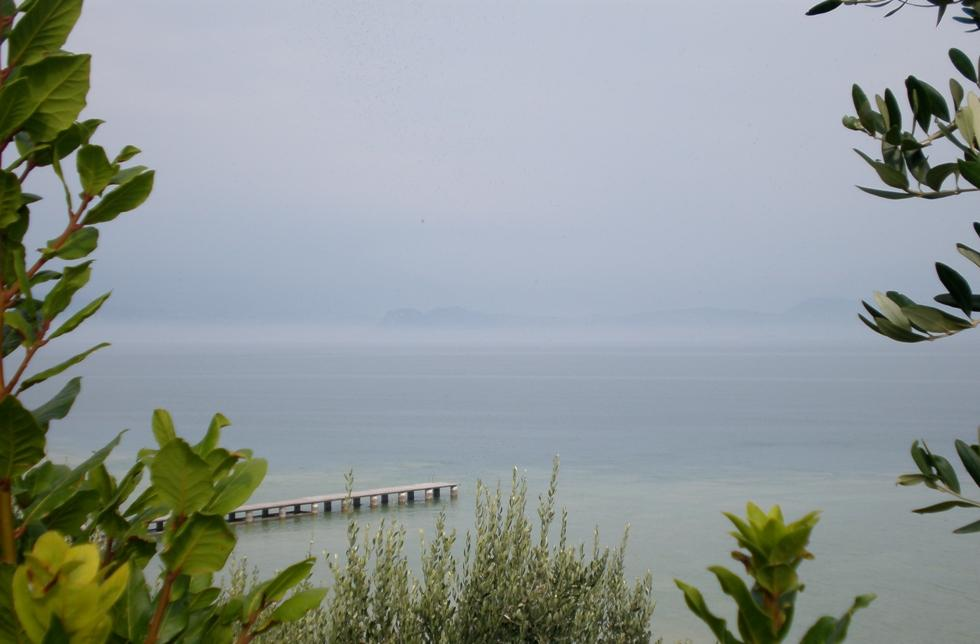
\includegraphics[scale=0.18]{./images/single_puzzle/pomeranz_805_3.jpg}} \\~\\
	Input Image~(a)~\cite{pomeranzBenchmarkImages} \\~\\
	\fbox{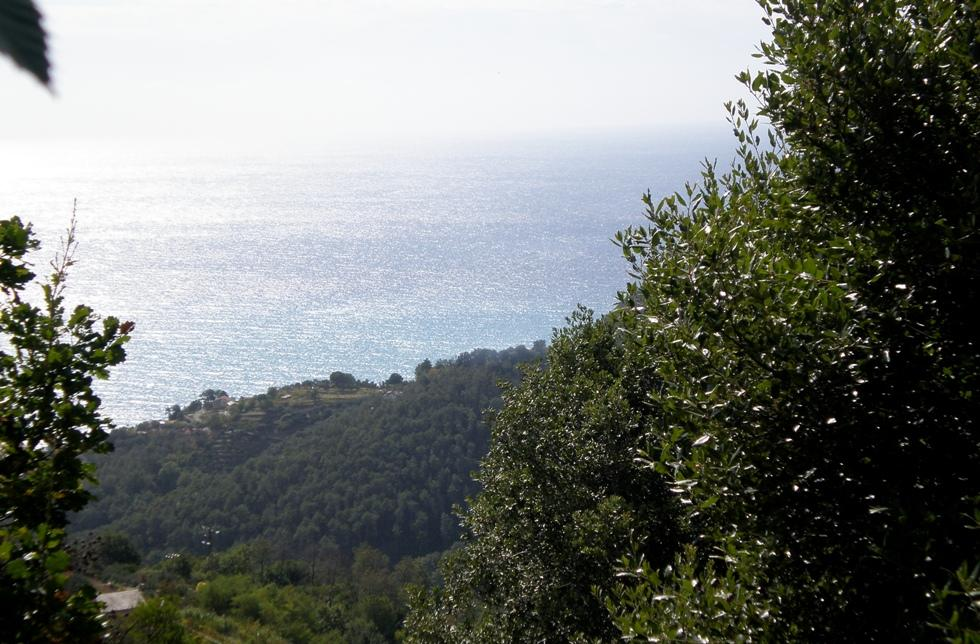
\includegraphics[scale=0.18]{./images/single_puzzle/pomeranz_805_12.jpg}} \\~\\
	Input Image~(b)~\cite{pomeranzBenchmarkImages} \\~\\
	\fbox{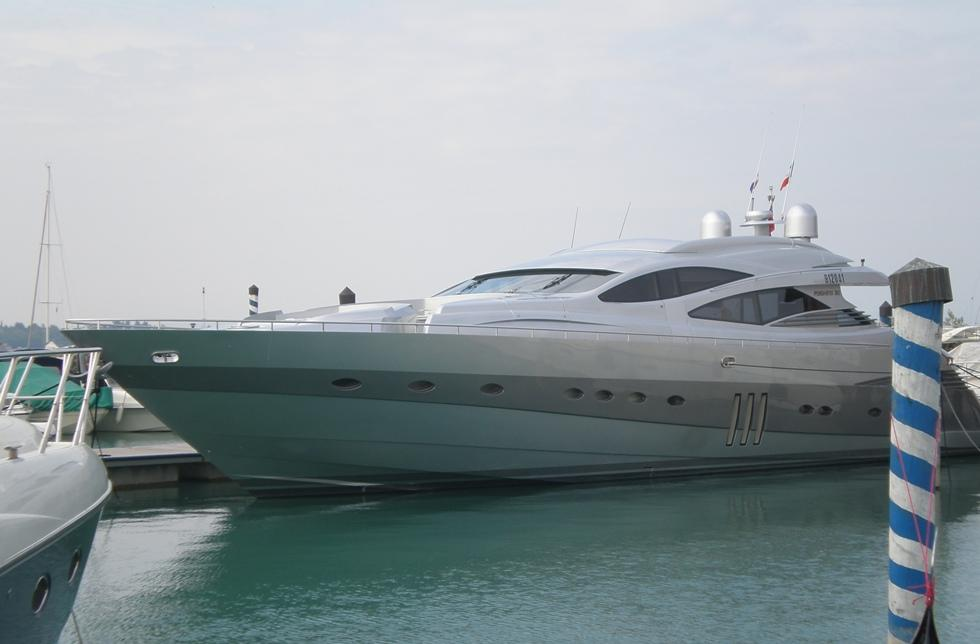
\includegraphics[scale=0.18]{./images/single_puzzle/pomeranz_805_16.jpg}} \\~\\
	Input Image~(c)~\cite{pomeranzBenchmarkImages} \\~\\
  \end{tabular}

\caption{805~Piece Images that were Incorrectly Identified by the Mixed-Bag Solver. Reproduced with Permission from Pomeranz \textit{et. al.}}
\label{fig:groundTruthSingleImageIncorrectlyIdentified}
\end{figure}

\begin{figure}
\centering
  \begin{tabular}{ >{\centering\arraybackslash}m{0.47\textwidth}  >{\centering\arraybackslash}m{0.47\textwidth} }

	\fbox{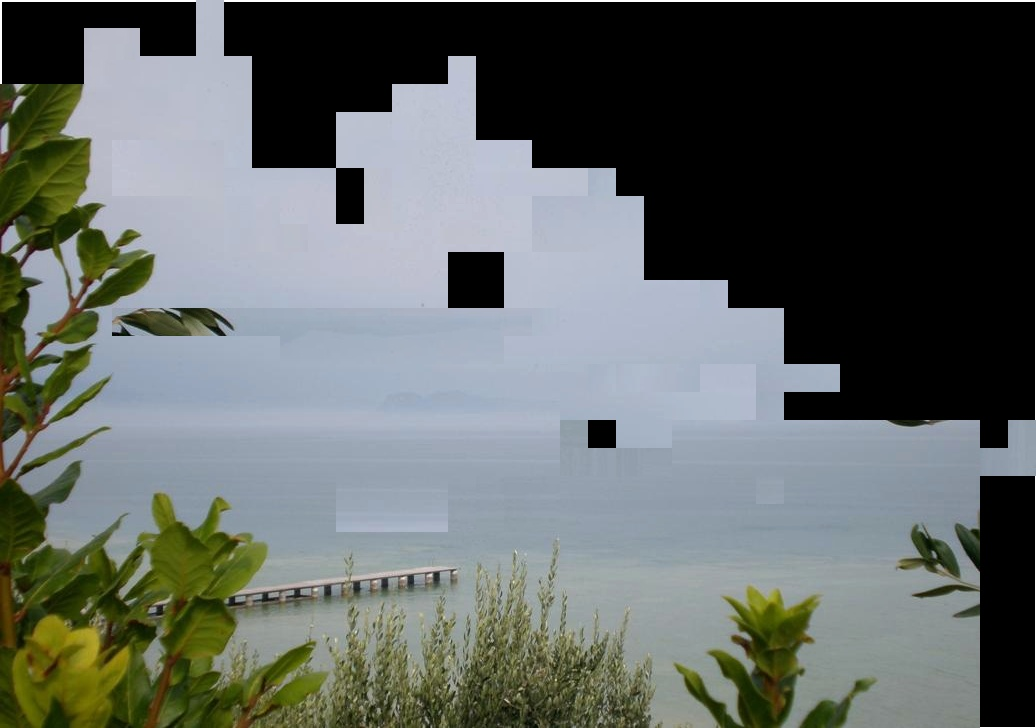
\includegraphics[scale=0.18]{./images/single_puzzle/reconstructed_805_3_01.jpg}} & \fbox{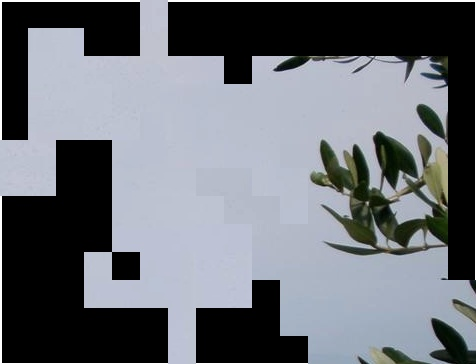
\includegraphics[scale=0.18]{./images/single_puzzle/reconstructed_805_3_02.jpg}} \\~\\
	Solver Output (a\hspace{0.1em}\textendash \hspace{0.08em}1) & Solver Output (a\hspace{0.1em}\textendash \hspace{0.1em}2) \\~\\
	
	\fbox{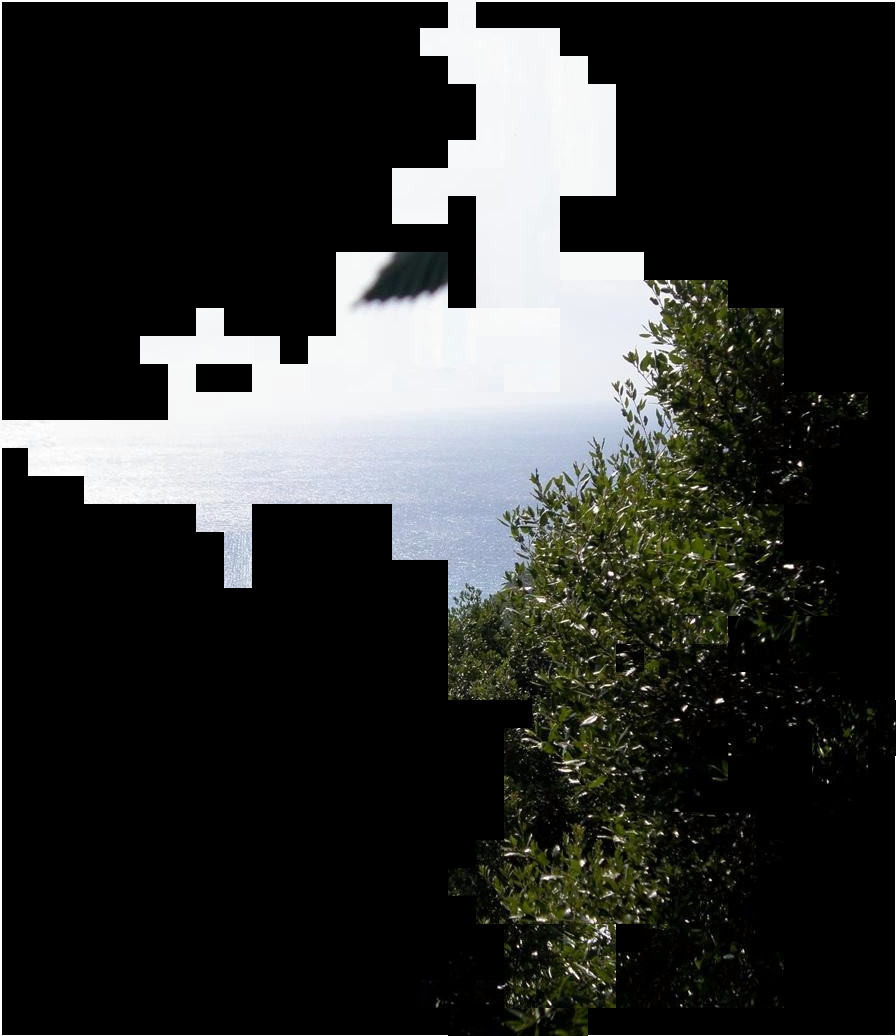
\includegraphics[scale=0.16]{./images/single_puzzle/reconstructed_805_12_02.jpg}} & \fbox{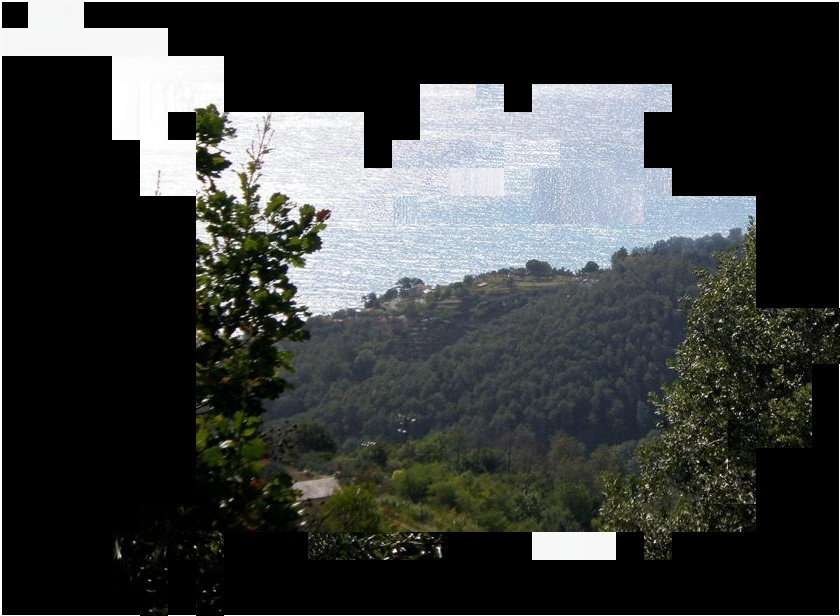
\includegraphics[scale=0.16]{./images/single_puzzle/reconstructed_805_12_01.jpg}} \\~\\
	Solver Output (b\hspace{0.15em}\textendash \hspace{0.08em}1) & Solver Output (b\hspace{0.1em}\textendash \hspace{0.1em}2) \\~\\
	
	\fbox{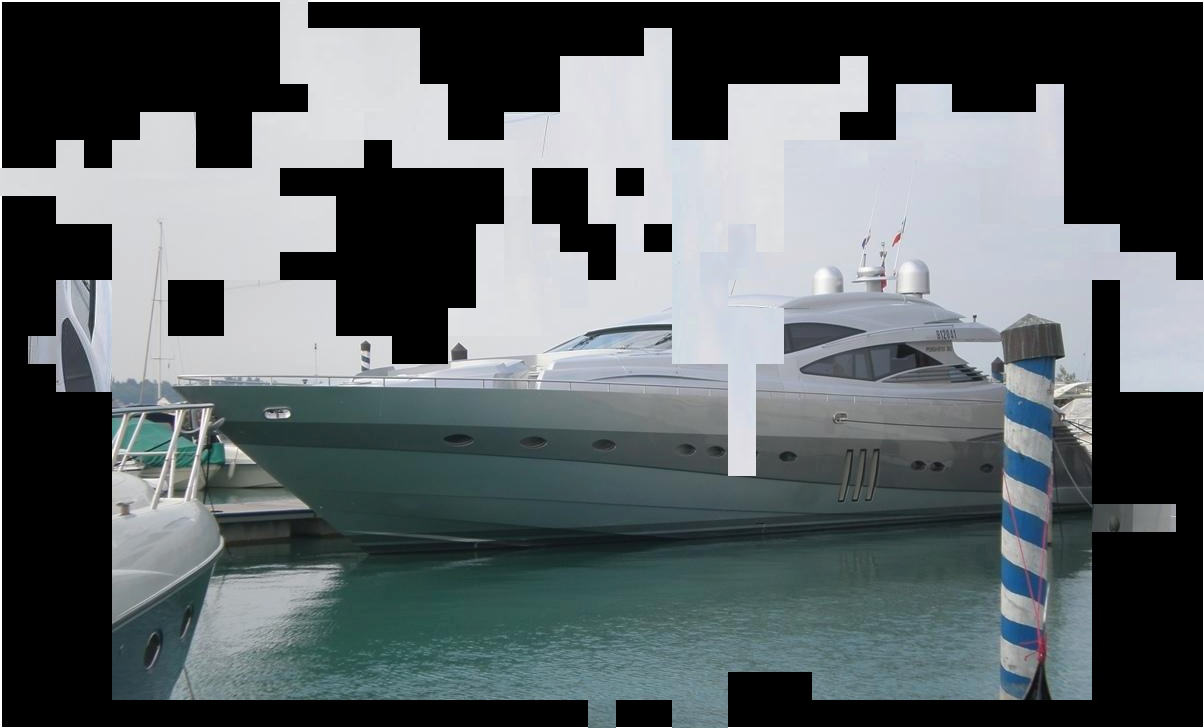
\includegraphics[scale=0.16]{./images/single_puzzle/reconstructed_805_16_01.jpg}} & \fbox{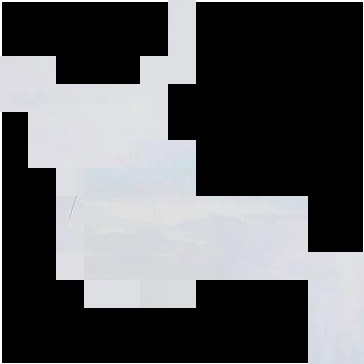
\includegraphics[scale=0.16]{./images/single_puzzle/reconstructed_805_16_02.jpg}} \\~\\
	Solver Output (c\hspace{0.15em}\textendash \hspace{0.08em}1) & Solver Output (c\hspace{0.15em}\textendash \hspace{0.1em}2) \\~\\
  \end{tabular}

\caption{Mixed-Bag Solver Outputs for the Incorrectly Identified Images}
\label{fig:mixedBagSolverOuputsSingleImageIncorrectlyIdentified}
\end{figure}
